\section{\label{sec:clas.dc}Drift Chambers (\abbr{DC})}

The primary subsystem of the \abbr{CLAS} detector is a collection of multi-wire proportional drift-chambers\cite{clas.dc} (\abbr{DC}) consisting of three layers in each of six sectors as shown in Fig.~\ref{fig:clas}. There is a toroidal magnetic field encompassing the middle layer which causes the charged particles to bend either directly toward or away from the beam-line. The magnetic field at regions 1 and 3 (inner and outer layers respectively) is relatively weak compared to region 2 as shown in Fig.~\ref{fig:clas.dc.torus.mag}. Therefore, the bending of the tracks is concentrated inside region 2 of the \abbr{DC} and the charge and momenta of the particles are determined by measuring the deflection angle of the tracks.

\begin{figure}\begin{center}
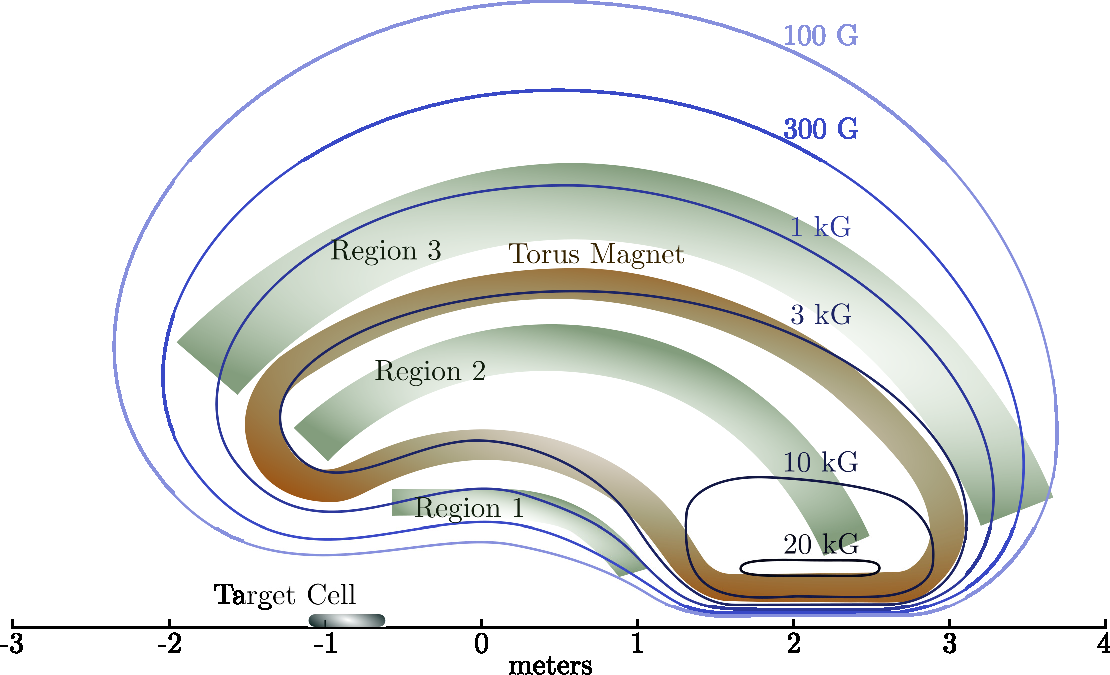
\includegraphics[width=\figwidth]{\figures/hall-b/torus_field_mag.pdf}
\caption[Magnetic Field Cross-sectional Magnitude]{\label{fig:clas.dc.torus.mag}Cross-section of the toroidal magnetic field at half current (1930~A). For \g12, the direction of the field was into the page and the 40~cm target center was placed at $-90$~cm from the \abbr{CLAS} center. Region 2 of the \abbr{DC} is located inside the region of the coils shown as the kidney shaped loop at about 3~kG.}
\end{center}\end{figure}

Each region of the \abbr{DC} consists of two \emph{superlayers} which contain six layers of evenly spaced 20~$\mu$m gold-plated tungsten \emph{sense wires} each surrounded by six 140~$\mu$m gold-plated aluminum alloy \emph{field wires}. The very first superlayer (region 1, superlayer 1) has only 4 layers due to space constraints. The field wires were kept at a high negative voltage (approximately $-1.5$~kV) while the sense wires were kept at a moderate positive voltage.

The gas used in the \abbr{DC} is 90\% argon and 10\% carbon-dioxide which is a non-flammable mixture that ionizes easily when charged particles above a certain energy pass through it. The ionized electrons cascade and drift toward the sense wires creating a signal that is amplified and passed through amplifier-discriminator boards (\abbr{ADB}s) and recorded by time-to-digital converters (\abbr{TDC}s). Due to budget considerations, there were no analog-to-digital (\abbr{ADC}) signals recorded from the \abbr{DC}. This could have provided information on the particles' energy loss as it traveled through the chambers, however, energy loss through other systems such as the \abbr{TOF} was available and used in this analysis, as discussed in Chapter~\ref{sec:analysis}.

\subsection{\label{sec:clas.dc.torus}Superconducting Toroidal Magnet}

The toroidal magnetic field used in \abbr{CLAS} is created by six kidney-shaped superconducting current loops\cite{clas} which are placed between the six sectors of the drift-chamber (\abbr{DC}) as shown in Fig.~\ref{fig:clas}. They each consist of 4 layers of 54 windings of aluminum-stabilized NbTi/Cu superconductor.

During the \g12 experiment, the magnets operated at a half-capacity current of 1930~A corresponding to a maximum field of about 20~kG. The magnetic field around the target area was low enough to allow for polarizing the target material though the \g12 target was unpolarized. The field was oriented such that positively charged particles bent away from the beam line, maximizing acceptance for these tracks. Increasing the current would improve the resolution of the detector, but sacrifice the acceptance for negatively charged particles. Since the physics goals of the \g12 proposals (see page~\pageref{sec:clas.g12}) involved many final state particles, both positive and negative, this balance of resolution and acceptance was used.

\begin{figure}\begin{center}
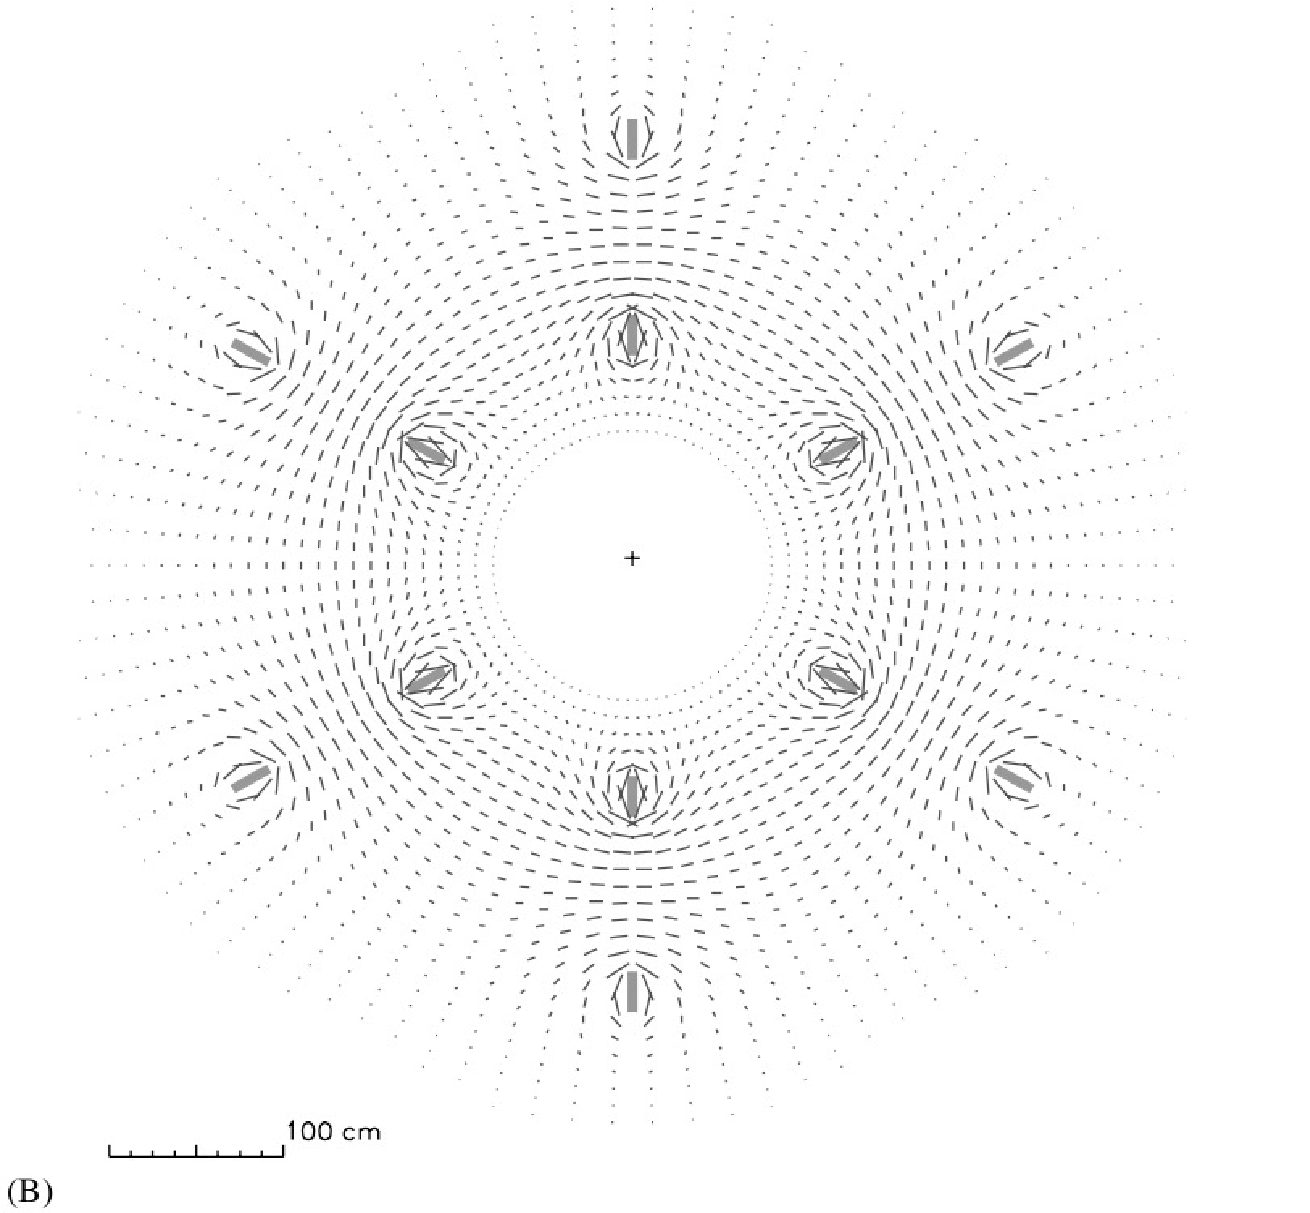
\includegraphics[width=0.8\figwidth]{\figures/hall-b/torus_field_cont.pdf}
\caption[Magnetic Field Line Diagram]{\label{fig:clas.dc.torus.cont}Toroidal magnetic field line diagram looking down-stream toward the \abbr{CLAS} detector. The field inside the windings indicated by the gray rectangles is in the counter-clockwise direction, and the field strength is concentrated in the region between the coils, see Fig.~\ref{fig:clas.dc.torus.mag}.}
\end{center}\end{figure}


